\scanpage{15}
\uline{Comparaison de classes fondamentales} analytiques ($\unsure{\simeq|=} \mathrm{alg}$) et topologiques ($=\mathrm{transc.}$).

$X$ variété \deleted{\unsure{analyti}} holomorphe

$Y$ ss-variété holomorphe de codim $p$ partout.

\[
\Omega_X^\bullet\quad\text{résolution de }\mathbb C
\]

\diagram{\resizebox{\linewidth}{!}{\begin{tikzcd}[ampersand replacement=\&,column sep=small,row sep=large]
\underline H^{2p}_Y(X,\mathbb Z) \arrow[r,hook,"{\substack{\mathrm{can}\\i}}"] \& \underline H^{2p}_Y(X,\mathbb Z)\otimes_{\mathbb Z}\mathbb C \arrow[r,"{\substack{\mathrm{can}\\\sim}}"] \& \underline H^{2p}_Y(X,\mathbb C) \arrow[r,"{\substack{\text{De Rham (i.e. can)}\\\sim}}"] \& \underline{\underline H}^{2p}_Y(X,\underline\Omega_X^\bullet) \& {}\\
\mathbb Z_Y \arrow[u,"{\substack{\sim\,P_{\mathrm{top}}^{\mathbb Z}\\\text{Poincaré topologique local}}}"] \arrow[r,hook] \& \overset{\deleted{\unsure{P_{\mathrm{top}}^{\mathbb Z}|P_{\mathrm{top}}}}}{\mathbb C_Y} \arrow[r,equal] \& \underset{\deleted{\unsure{\underline H^{2p}_Y(X,\underline\Omega_X^\bullet)|\underline H^p_Y(X,\underline\Omega_X^\bullet)}}}{\mathbb C_Y} \arrow[u,"{\sim\,P_{\mathrm{top}}^{\mathbb C}}"] \arrow[r,"{\frac{1}{(2i\pi)^p}}"'] \& \mathbb C_Y \arrow[u,"{\sim\,P_{\mathrm{an}}^{\unsure{\mathbb C|\mathbb Z|\Omega}}}"] \arrow[r,"{\text{\uuline{résidu}}}"'] \& \underline H^p_Y(X,\underline\Omega_X^p) \arrow[ul,"{\text{suite spectrale}}"']
\end{tikzcd}}}

\margin{\uline{Poincaré analytique local} [défini par voie ess. alg.] si $f_1\ldots f_p$ est un syst. d'équations locales de $Y$, on prend la section $\frac{df_1}{f_1}\wedge\ldots\wedge\frac{df_p}{f_p}$ de $\underline H^p_Y(\underline\Omega^p_X)$}

On est ramené au cas où $Y$ est réduit à un pt $a$ (prendre une \deleted{section} $X'^{n-p}$ transversale à $Y$ en un pt) et par cup-produit au cas où $X$ est de dim $1$, si on veut un disque de centre $\unsure{a|x}$

[N.B. à priori, cet argument prouve déjà qu'il \deleted{le} \inserted{existe un} multiplicateur de la forme $\lambda^p$, $\lambda\in\mathbb C^*$ étant indépendant de $X,Y,p$]. Alors on a

\diagram{\resizebox{\linewidth}{!}{\begin{tikzcd}[ampersand replacement=\&,row sep=small,column sep=small]
H^1(X-a,\mathbb Z) \arrow[r] \arrow[d,phantom,"{\rotatebox{90}{$\simeq$}}"] \& H^1(X-a,\mathbb C) \arrow[r,"\sim"] \arrow[d,phantom,"{\rotatebox{90}{$\simeq$}}"] \& \underline{\underline H}^1(X-a,\underline\Omega_X^\bullet) \arrow[d,phantom,"{\rotatebox{90}{$\simeq$}}"] \& {}\\
H^2_a(X,\mathbb Z) \arrow[r] \& H^2_a(X,\mathbb C) \arrow[r,"\sim"] \& \underline{\underline H}^2_a(X,\underline\Omega_X^\bullet) \& {}\\
\mathbb Z \arrow[u,"{\sim\,P_t^{\mathbb Z}}"] \arrow[r] \& \mathbb C \arrow[u,"{P_t^{\mathbb C}}"] \arrow[r,"\lambda"] \& \mathbb C \arrow[u,"{P_{\mathrm{an}}^{\mathbb C}}"] \arrow[r] \& H^1_a(X,\Omega^1_X)\quad\frac{dz}{z} \arrow[ul,"\sim"']
\end{tikzcd}}}
\figure{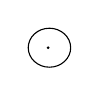
\begin{tikzpicture}[scale=.55]\draw (0,0) ellipse (.49 and .45);\fill (-.03,0) circle (.035);\end{tikzpicture}}
% archive sheet number: 14
